\subsection{Implementación en PCB}

Una vez definidos todos los circuitos que componen a la plataforma, se llega a un total de {\Medium 197 componentes} discretos con decenas de empaquetados distintos, que deben todos ser posicionados en una placa de circuito impreso doble faz del menor tamaño posible. El resultado final de la plaqueta, con todos sus componentes (exceptuando los disipadores térmicos de los transistores y diodos de potencia) se observa en la figura \ref{fig:PCB_3D}.\\

\begin{figure}[h]
    \centering
    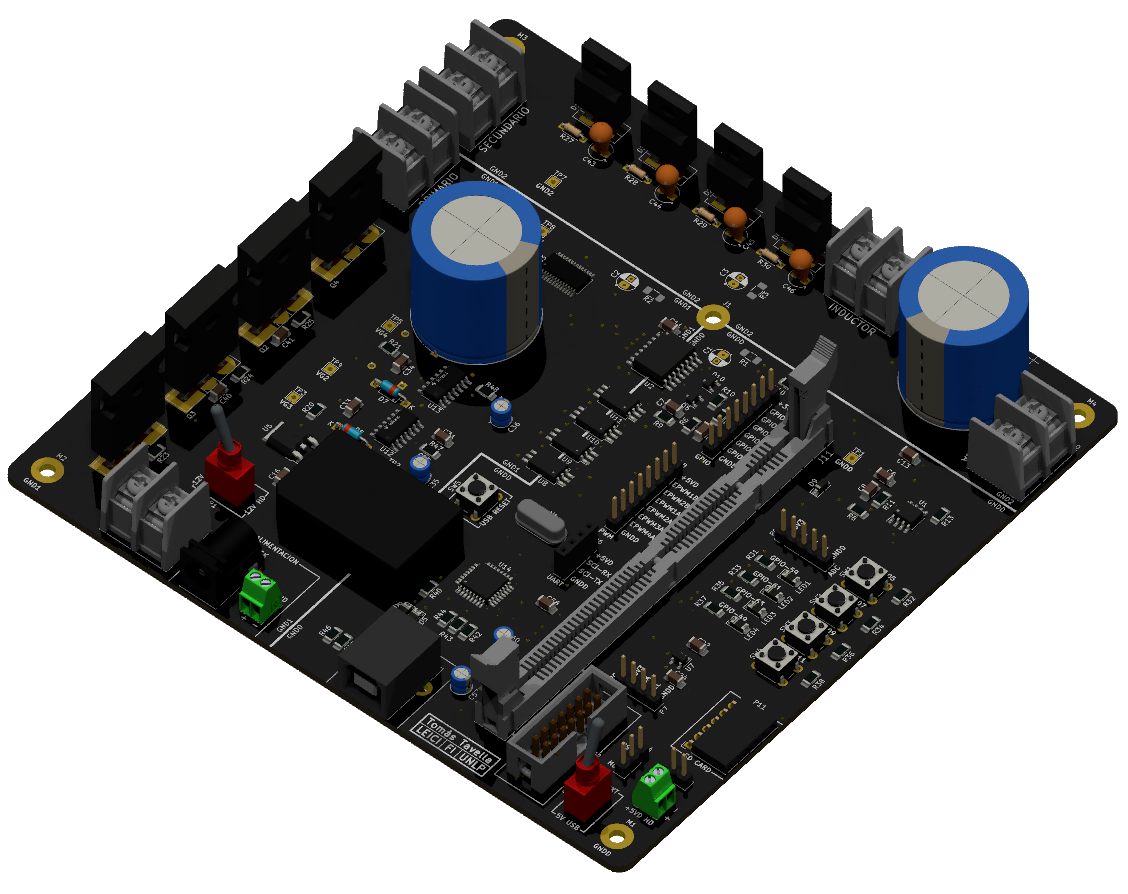
\includegraphics[scale=0.34]{Imagenes/PCB 3D Raytracing.png}
    \caption{Modelo tridimensional de la implementación en PCB de la plataforma con todos sus componentes, vista desde la parte superior.}
    \label{fig:PCB_3D}
\end{figure}

Para comenzar, se va a realizar un listado de todos los componentes, clasificados según sus distintos encapsulados y sus \textit{footprints} correspondientes (es la \quotes{huella} de cada componente sobre la plaqueta). Una vez establecido este listado, se procede a detallar el proceso de diseño de la placa de circuito impreso, comenzando por el posicionamiento de todos los componentes de la forma más compacta posible respetando la sepación de tierras y dando el espacio necesario para el ruteo de pistas. Finalmente se conectan todos los componentes según indica el esquema circuital de la plataforma, y se realizan verificaciones finales previo a la generación de los archivos de fabricación definitivos.\\

\subsubsection{Listado de Componentes}

En la tabla \ref{tabla:componentes} de la próxima página se presenta un listado de todos los componentes de la placa de circuito impreso, separados según su tipo de empaquetado, ya sea de montaje superficial (SMD) o de tipo through-hole (THT). Esto incluye circuitos integrados como los distintos sensores, resistencias y capacitores de todos los circuitos, transistores y diodos de potencia y auxiliares, y todos los distintos conectores de alimentación y señal.\\

\setlength{\tabcolsep}{8pt}
\renewcommand{\arraystretch}{1.45}
\begin{table}[H]
\begin{center}
    \begin{tabular}{llrl}
        & {\SemiBold Empaquetado} & {\SemiBold Cantidad} & {\SemiBold Descripción}\\
        \hline
        \multirow{14}{*}{\SemiBold SMD} & 1206 & \num{85} & Capacitores, Resistores y LED\\
        & 1210 & \num{1} & Capacitor Tantalio\\
        & 3 x 5.4 \unit{\milli\metre} & \num{2} & Capacitores Aluminio\\
        & 2512 & \num{1} & Resistor Shunt\\
        & SOIC-8 & \num{3} & Sensor Hall y otros\\
        & SOIC-16W & \num{1} & Aislador ISO7242C\\
        & HTSSOP-28 & \num{1} & Sensor LM5056A\\
        & SSO-6 & \num{4} & Optoacoplador ACPL-P480\\
        & SO-14 & \num{2} & Drivers 2ED21834-S06J\\
        & LQFP-32 & \num{1} & FTDI FT232BL\\
        & SOD-123 & \num{1} & Diodo Schottky\\
        & SOT-23 & \num{3} & Diodos Schottky y Transistores\\
        & SOT-23-5 & \num{2} & Reguladores Lineales\\
        & TO-252-2 & \num{1} & Regulador Lineal\\
        \hline
        \multirow{19}{*}{\SemiBold THT} & D25\unit{\milli\metre} & \num{2} & Capacitores Electrolíticos \SI[]{680}[]{\micro\farad}\\
        & D4\unit{\milli\metre} & \num{7} & Capacitores Electrolíticos\\
        & D4,5\unit{\milli\metre} & \num{4} & Capacitores Tantalio\\
        & D1,6\unit{\milli\metre} x L3,6\unit{\milli\metre} & \num{4} & Resistores\\
        & TO-247AC & \num{4} & Transistores IRFP150\\
        & TO-220 & \num{4} & Diodos MUR860\\
        & DIP-24 & \num{1} & Fuente Aislada THB3-1211\\
        & DO-35 & \num{4} & Diodos\\
        & HC-18 & \num{1} & Cristal\\
        & DIMM100 & \num{1} & Conector DIMM para DSC\\
        & DCJ200-10A & \num{1} & Barrel Jack\\
        & USB-B & \num{1} & Conector USB-B Hembra\\
        & Degson Screw Terminal & \num{5} & Conectores Pila, Carga, etc.\\
        & Phoenix Contact 2P & \num{2} & Conectores 5V y 12V Externo\\
        & Pulsador P6\unit{\milli\metre} & \num{5} & Pulsadores\\
        & Pin Header P2,54\unit{\milli\metre} & \num{34} & Tiras de Pines\\
        & Pin Header P2,54\unit{\milli\metre} 2x7 & \num{1} & Conector J-TAG\\
        & Pin Socket P2,54\unit{\milli\metre} & \num{6} & Conectores Pines Hembra\\
        & Switch 3P P2,54\unit{\milli\metre} & \num{2} & Interruptor de 3 Polos\\
        \hline
        {\SemiBold Total} & & {\SemiBold 197} &
    \end{tabular}
    \caption{Lista completa de componentes de la plataforma, clasificados según su tipo y modelo de encapsulado.}
    \label{tabla:componentes}
\end{center}
\end{table}

Ahora, todos estos componentes se deben posicionar de manera compacta en la placa doble faz de aproximadamente \SI[]{15}[]{\centi\metre} de lado, y conectarse de acuerdo a los circuitos presentados en la sección anterior, teniendo en cuenta las consideraciones de ancho de pista y conexión de tierras.\\

\subsubsection{Ubicación y Disposición de Circuitos}

Para ubicar los componentes en la plaqueta, se deben agrupar claramente en tres regiones distintas: los componentes que se conectan a la referencia digital GND\textsubscript{D}, los que se conectan a la referencia del primario GND\textsubscript{1}, y los que se conectan a la referencia del secundario GND\textsubscript{2}. Existe una pequeña selección de componentes, como por ejemplo el aislador ISO7242C, que se encuentran entre dos de estas zonas, por formar parte del circuito de aislación de señal de la plataforma.\\ 

En la figura \ref{fig:PCB_cobre}, que corresponde a ambas capas de cobre de la placa de circuito impreso, se pueden observar claramente las 3 distintas regiones en las que se divide, con GND\textsubscript{1} a la izquiera, GND\textsubscript{2} en la parte superior y GND\textsubscript{D} a la derecha. Adicionalmente, en \ref{fig:PCB_cobre}a están marcadas las regiones de la placa que se corresponden a cada uno de los seis bloques de la plataforma de la figura \ref{fig:plataforma_det}. Vamos a tratar la disposición de los circuitos de cada una de estas regiones a continuación.\\

\paragraph{Región 1 - Convertidor CC-CC Conmutado}

Esta región contiene todos los componentes que forman parte del circuito del convertidor CC-CC de puente completo de la plataforma de la figura \ref{fig:fullbridge}, con partes conectadas a la tierra del primario GND\textsubscript{1} y otras partes a la tierra del secundario GND\textsubscript{2}, causado por la presencia de un transformador que provee aislación galvánica entre primario y secundario.\\

Abajo a la izquierda de esta región se encuentran los cuatro transistores MOSFET de potencia modelo IRFP150 (encapsulado THT tipo TO-247AC) que conforman el puente del lado primario, y hacia arriba se pueden ver los cuatro diodos de potencia modelo MUR860 (encapsulado THT tipo TO-220) del puente del lado secundario. Estos componentes se posicionaron deliberadamente en los bordes de la placa, ya que requieren grandes disipadores metálicos para manejar efectivamente el calor generado por los niveles de potencia que manejan.\\

\begin{figure}[h]
    \centering
    \begin{subfigure}
        \centering
        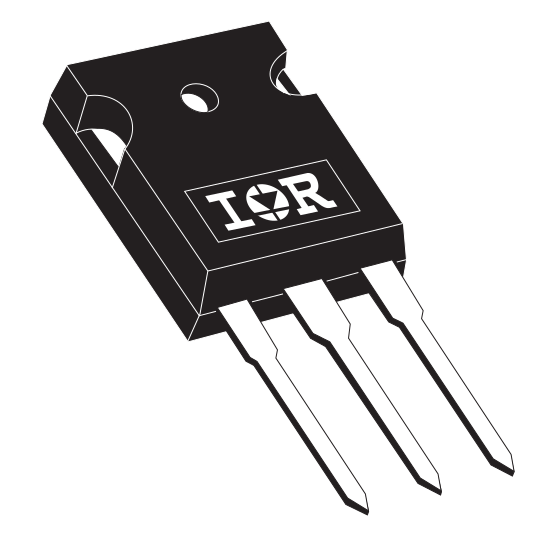
\includegraphics[width=0.18\textwidth]{Imagenes/IRFP150-TO247AC.png}
    \end{subfigure}
    \hspace{2em}
    \begin{subfigure}
        \centering
        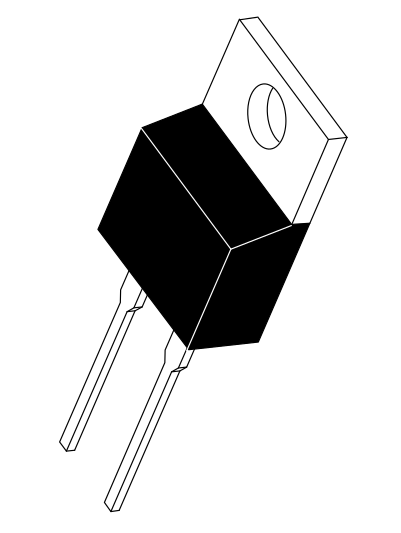
\includegraphics[width=0.13\textwidth]{Imagenes/MUR860.png}
    \end{subfigure}
    \caption{De izquierda a derecha: encapsulados tipo TO-247AC y TO-220, correspondientes a los transistores IRFP150 y diodos MUR860.}
    \label{fig:IRFP150-MUR860}
\end{figure}

También se pueden ver en esta región dos marcas circulares grandes, que corresponden a los capacitores electrolíticos de filtro a la entrada y salida del convertidor, en paralelo a la pila de hidrógeno y a la carga variable respectivamente. Estos son capacitores de valores elevados (ambos de \SI[]{680}[]{\micro\farad}), y en particular el de salida debe soportar tensiones pico que pueden superar los \SI[]{120}[]{\volt}. Por estas razones, se seleccionaron capacitores blindados de \SI[]{200}[]{\volt} de tensión máxima, que se consiguen en encapsulados muy grandes, en nuestro caso de \SI[]{25}[]{\milli\metre} de diámetro y \SI[]{40}[]{\milli\metre} de altura, similar al que se observa en la figura \ref{fig:CapFiltro}.\\

\begin{figure}[h]
    \centering
    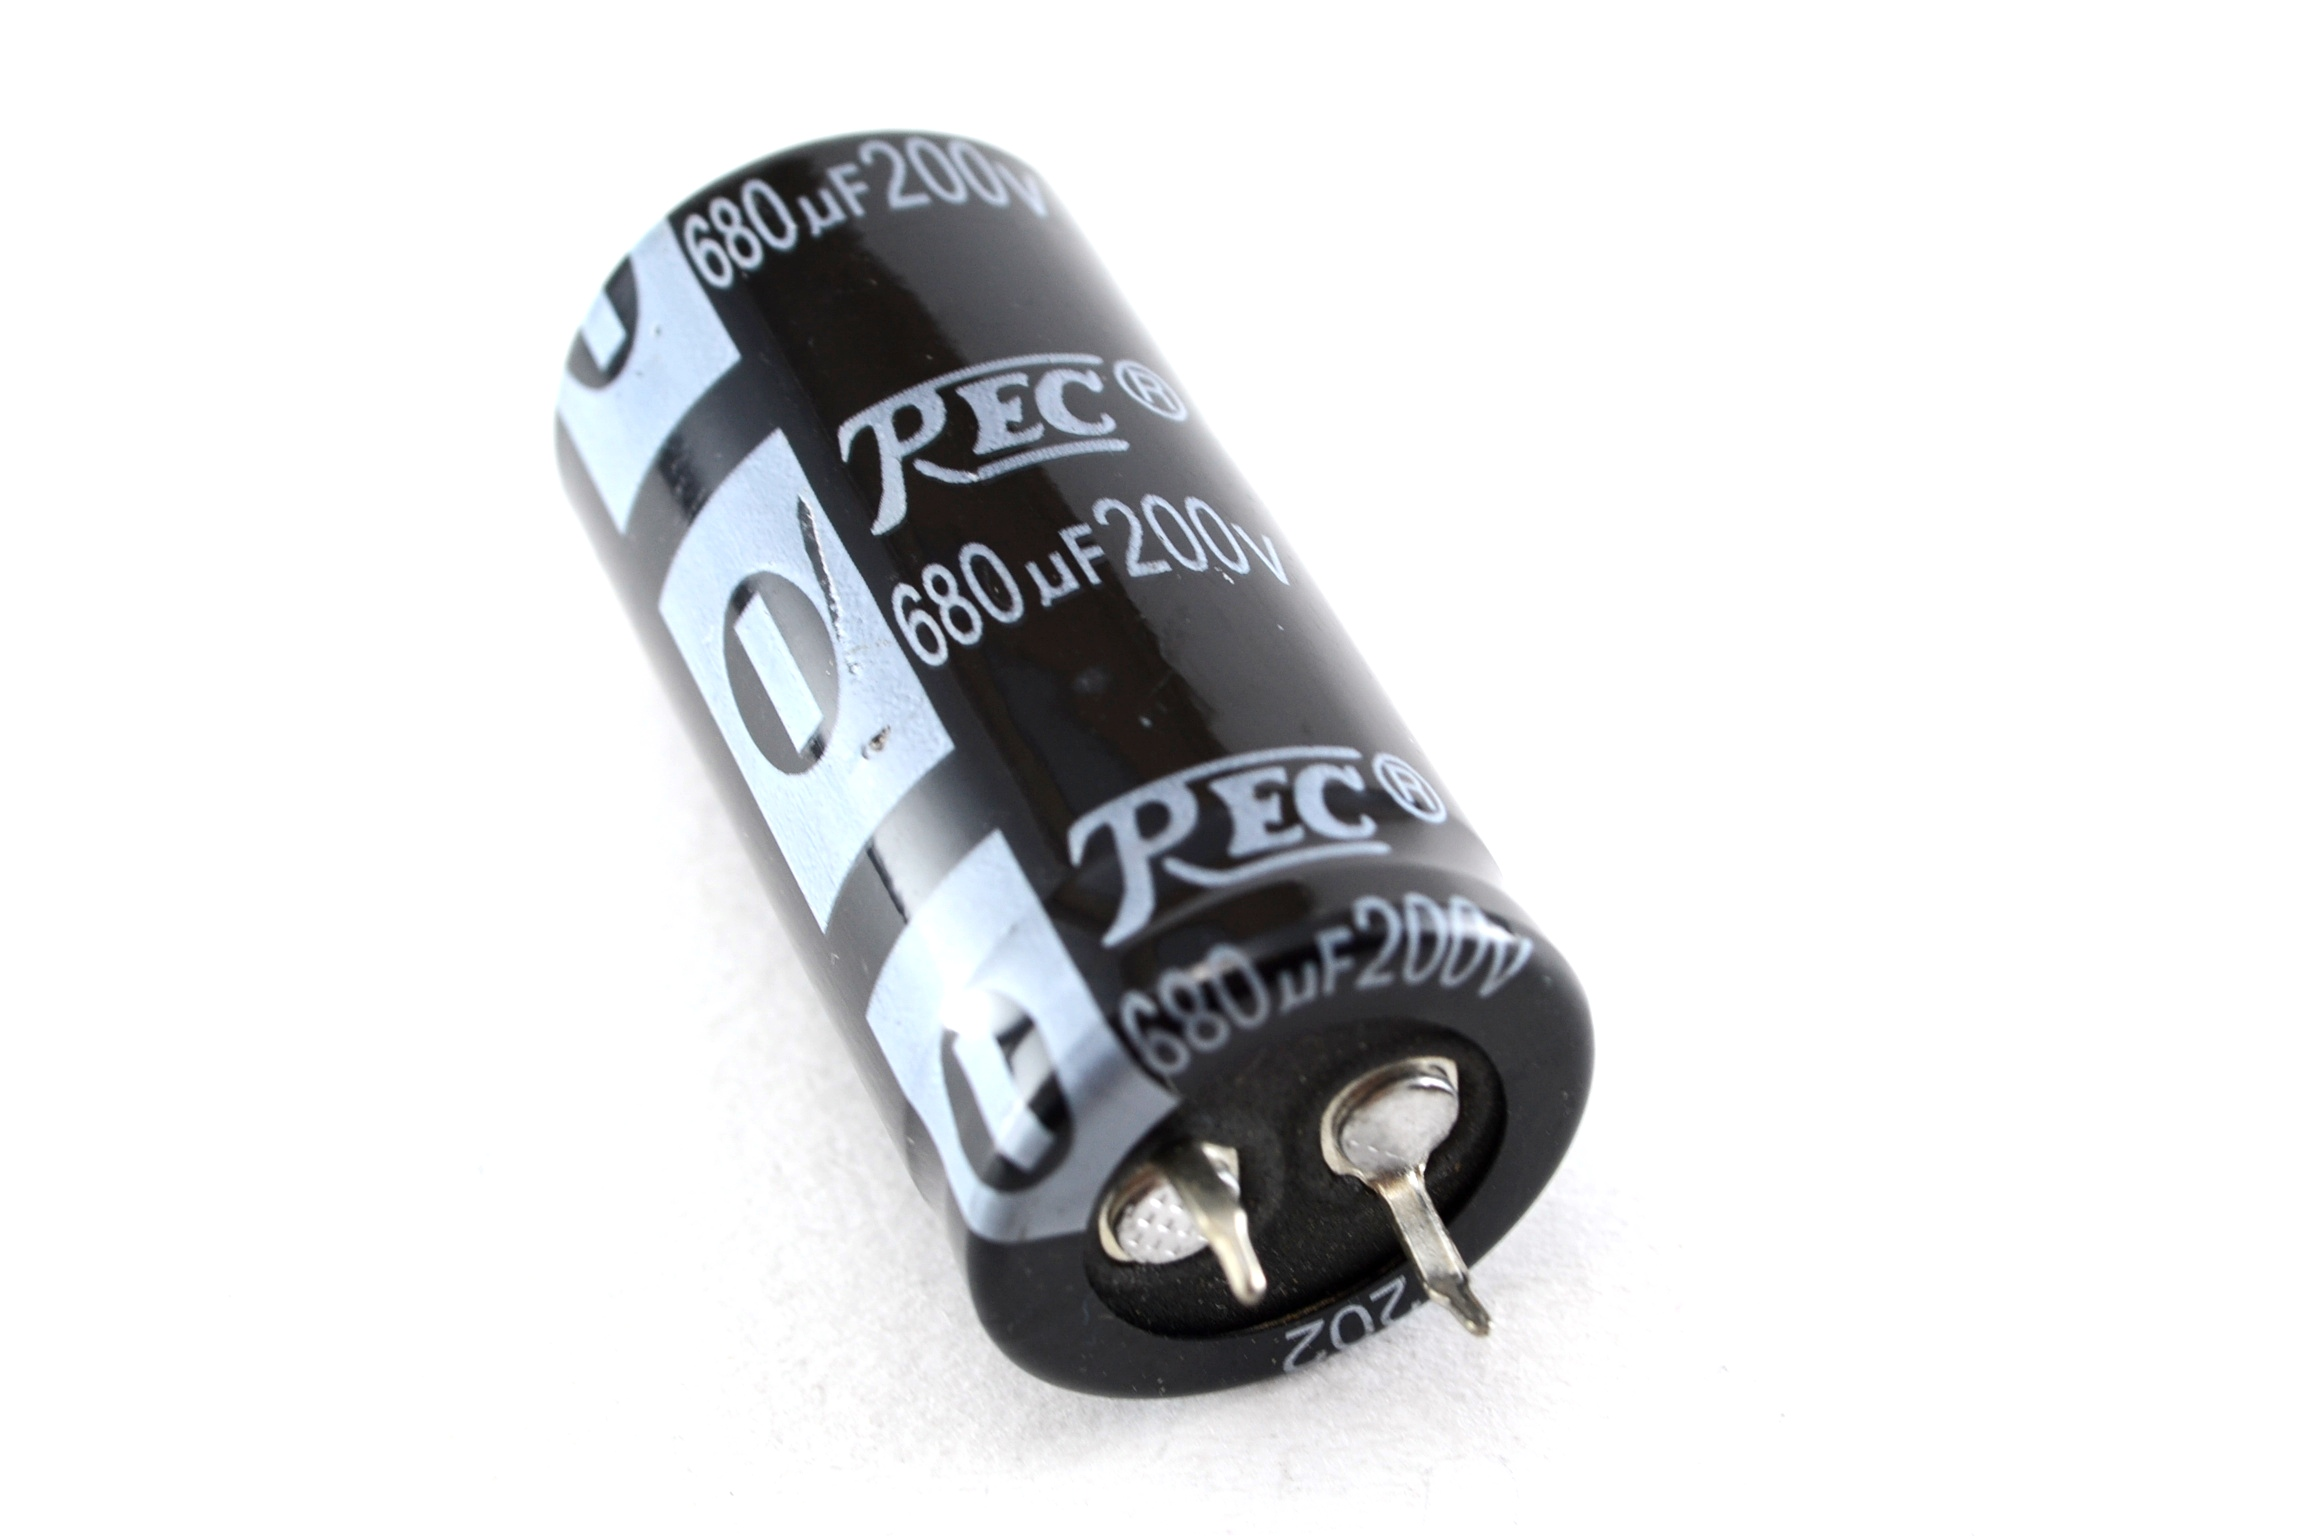
\includegraphics[scale=0.3]{Imagenes/Capacitor Blindado.jpg}
    \caption{Capacitor electrolítico blindado de \SI[]{25}[]{\milli\metre} de diámetro, similar al utilizado en la plataforma.}
    \label{fig:CapFiltro}
\end{figure}

El inductor del filtro de salida y el transformador de alta frecuencia no se encuentran directamente sobre la placa, dado que son elementos de grandes dimensiones y aumentarían el tamaño de la PCB considerablemente si se colocaran en la misma. Por esta razón, se colocan terminales de alta tensión y corriente para conectar el primario y secundario del transformador, además del inductor de salida. Se utilizan dos conectores adicionales para conectar la pila de hidrógeno a la entrada y la carga variable a la salida.\\

En la pista que conecta el terminal positivo de la pila de hidrógeno con el capacitor de filtro, se coloca la resistencia shunt de \SI[]{4}[]{\milli\ohm} utilizada por el sensor LM5056A para medir la corriente de pila. A diferencia del resto de las resistencias SMD, el shunt utiliza un encapsulado de dimensiones 2512, es decir \SI[]{6.4}[]{\milli\metre} x \SI[]{3}[]{\milli\metre}. Esto es necesario para poder realizar apropiadamente la conexión Kelvin de cuatro cables para la medición de la tensión shunt $V_S$: se conectan los cables que llevan la corriente por separado de los cables utilizados para medir la tensión, como se ve en la figura \ref{fig:ConexionShunt}.\\

\begin{figure}[h]
    \centering
    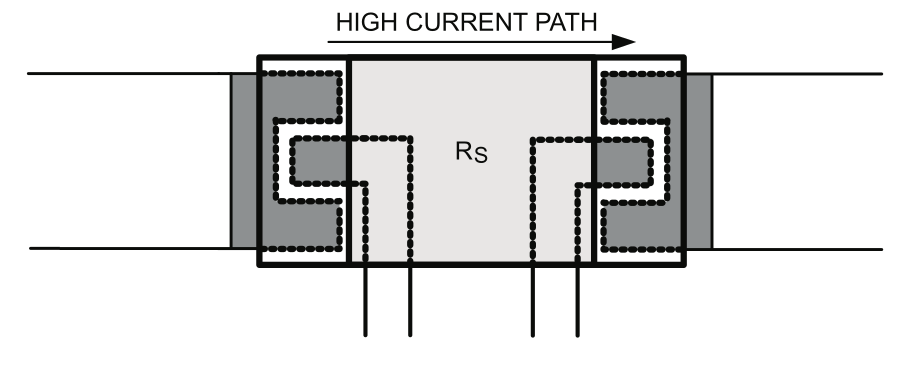
\includegraphics[scale=0.9]{Imagenes/Conexion Kelvin.png}
    \caption{Esquema de la conexión Kelvin de cuatro cables para la medición de la caida de tensión en la resistencia shunt.}
    \label{fig:ConexionShunt}
\end{figure}

\subparagraph{Anchos de Pista}

Utilizando la ecuación \ref{eq:IPC2221} establecida por la norma IPC-2221, se calculan los anchos de pistas necesarios teniendo en cuenta el grosor H fijo de \SI[]{0.035}[]{\milli\metre} y estableciendo la máxima elevación de temperatura de pista en \SI[]{20}[]{\celsius}.\\

En el lado primario del convertidor, la máxima corriente que la pila de hidrógeno puede proveer es de aproximadamente \SI[]{10}[]{\ampere}, de manera que el ancho de pista del lado primario debe cumplir con el siguiente requerimiento:

\begin{equation}\label{eq:Wprimario}
    W_{primario} > \SI[]{4.72}[]{\milli\metre}
\end{equation}

Y en el lado secundario, dada la potencia máxima de \SI[]{300}[]{\watt} y la tensión de salida fija de \SI[]{75}[]{\volt}, la corriente máxima que circulará es de aproximadamente \SI[]{4}[]{\ampere}, por lo que el requerimiento de ancho de pista resulta:

\begin{equation}\label{eq:Wsecundario}
    W_{secundario} > \SI[]{1.34}[]{\milli\metre}
\end{equation}

Con estos requerimientos en cuenta, los tamaños finales de las pistas de primario y secundario están resumidos en la siguiente tabla.\\

\setlength{\tabcolsep}{8pt}
\renewcommand{\arraystretch}{1.5}
\begin{table}[H]
\begin{center}
    \begin{tabular}{lr}
        & {\SemiBold Ancho de Pista}\\
        \hline
        \Medium Primario & \SI[]{5}[]{\milli\metre}\\
        \Medium Secundario & \SI[]{2}[]{\milli\metre}
    \end{tabular}
    \caption{Resumen de anchos de pista del circuito del convertidor CC-CC Conmutado.}
    \label{tabla:anchos_convertidor}
\end{center}
\end{table}

\paragraph{Región 2 - Circuito Driver}

\lipsum[1]\\

\paragraph{Región 3 - Sistema de Medición}

\lipsum[2]\\

\paragraph{Región 4 - Etapa de Aislación de Señal}

\lipsum[3]\\

\paragraph{Región 5 - Sistema de Control}

\lipsum[4]\\

\paragraph{Región 6 - Circuito de Alimentación}

\lipsum[5]\\

\newpage\afterpage{\blankpage}

\begin{figure}[H]
    \centering
    \subfigure[Capa de cobre frontal, con los distintos bloques de la plataforma indicados.]{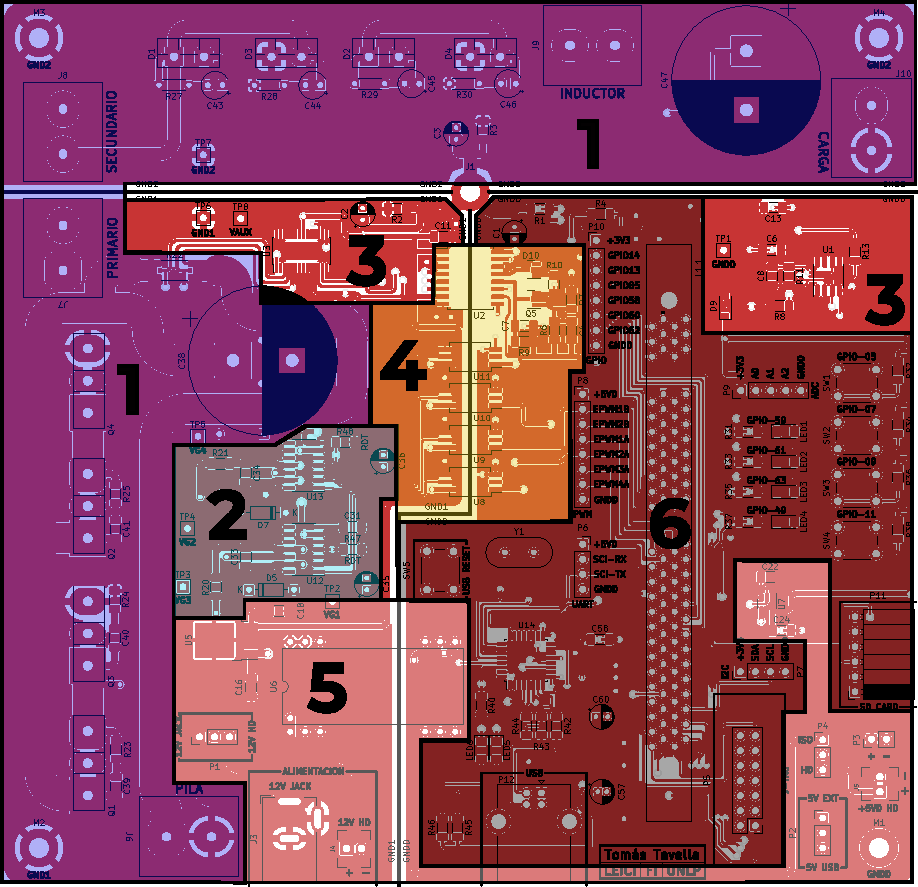
\includegraphics[scale=0.8]{Imagenes/PCB Front - SubCircuitos.pdf}}\\
    \subfigure[Capa de cobre trasera, con las tres distintas puestas a tierra.]{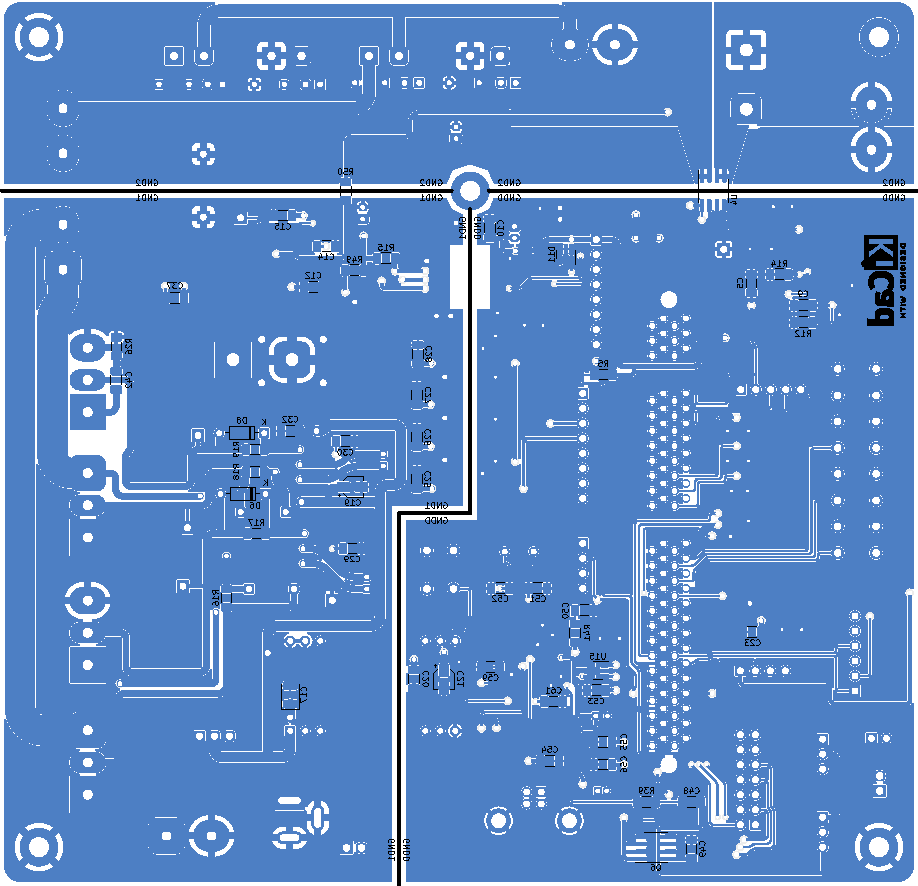
\includegraphics[scale=0.8]{Imagenes/PCB Back Layer.pdf}}%
    \caption{Diagrama de las distintas capas de cobre de la PCB.}
    \label{fig:PCB_cobre}
\end{figure}